\documentclass{beamer}
\mode<presentation>
\usepackage{amsmath}
\usepackage{amssymb}
%\usepackage{advdate}
\usepackage{adjustbox}
\usepackage{subcaption}
\usepackage{enumitem}
\usepackage{multicol}
\usepackage{mathtools}
\usepackage{listings}
\usepackage{url}
\def\UrlBreaks{\do\/\do-}
\usetheme{Boadilla}
\usecolortheme{lily}
\setbeamertemplate{footline}
{
  \leavevmode%
  \hbox{%
  \begin{beamercolorbox}[wd=\paperwidth,ht=2.25ex,dp=1ex,right]{author in head/foot}%
    \insertframenumber{} / \inserttotalframenumber\hspace*{2ex} 
  \end{beamercolorbox}}%
  \vskip0pt%
}
\setbeamertemplate{navigation symbols}{}

\providecommand{\nCr}[2]{\,^{#1}C_{#2}} % nCr
\providecommand{\nPr}[2]{\,^{#1}P_{#2}} % nPr
\providecommand{\mbf}{\mathbf}
\providecommand{\pr}[1]{\ensuremath{\Pr\left(#1\right)}}
\providecommand{\qfunc}[1]{\ensuremath{Q\left(#1\right)}}
\providecommand{\sbrak}[1]{\ensuremath{{}\left[#1\right]}}
\providecommand{\lsbrak}[1]{\ensuremath{{}\left[#1\right.}}
\providecommand{\rsbrak}[1]{\ensuremath{{}\left.#1\right]}}
\providecommand{\brak}[1]{\ensuremath{\left(#1\right)}}
\providecommand{\lbrak}[1]{\ensuremath{\left(#1\right.}}
\providecommand{\rbrak}[1]{\ensuremath{\left.#1\right)}}
\providecommand{\cbrak}[1]{\ensuremath{\left\{#1\right\}}}
\providecommand{\lcbrak}[1]{\ensuremath{\left\{#1\right.}}
\providecommand{\rcbrak}[1]{\ensuremath{\left.#1\right\}}}
\theoremstyle{remark}
\newtheorem{rem}{Remark}
\newcommand{\sgn}{\mathop{\mathrm{sgn}}}
\providecommand{\abs}[1]{\left\vert#1\right\vert}
\providecommand{\res}[1]{\Res\displaylimits_{#1}} 
\providecommand{\norm}[1]{\lVert#1\rVert}
\providecommand{\mtx}[1]{\mathbf{#1}}
\providecommand{\mean}[1]{E\left[ #1 \right]}
\providecommand{\fourier}{\overset{\mathcal{F}}{ \rightleftharpoons}}
%\providecommand{\hilbert}{\overset{\mathcal{H}}{ \rightleftharpoons}}
\providecommand{\system}{\overset{\mathcal{H}}{ \longleftrightarrow}}
	%\newcommand{\solution}[2]{\textbf{Solution:}{#1}}
%\newcommand{\solution}{\noindent \textbf{Solution: }}
\providecommand{\dec}[2]{\ensuremath{\overset{#1}{\underset{#2}{\gtrless}}}}
\newcommand{\myvec}[1]{\ensuremath{\begin{pmatrix}#1\end{pmatrix}}}
\let\vec\mathbf

\lstset{
%language=C,
frame=single, 
breaklines=true,
columns=fullflexible
}

\numberwithin{equation}{section}

\title{Matgeo-7-7.3-5}
\author{Arnav Mahishi \\ Dept. of Electrical Engg.\\IIT Hyderabad.}

\date{\today} 
\begin{document}

\begin{frame}
\titlepage
\end{frame}
\section*{Outline}
\begin{frame}
\tableofcontents
\end{frame}
\section{Problem}
\begin{frame}
\frametitle{Problem Statement}
If a circle passes through the points $\brak{0,0}$,$\brak{a,0}$,and $\brak{0,b}$ then find the coordinates of its centre.
\end{frame}

%\subsection{Literature}
\section{Solution}
\subsection{Input Parameters}
\begin{frame}
\frametitle{Input Parameters}
\begin{table}[]
    \centering
    \begin{tabular}[10pt]{|c|c|}
    \hline
    \textbf{input} & \textbf{value}\\ 
    \hline
    $x_1$&$\myvec{0\\0}$\\
    \hline 
    $x_2$&$\myvec{a\\0}$\\
    \hline 
    $x_3$&$\myvec{0\\b}$\\
    \hline
    \end{tabular}
    \caption{Input Parameters}
    \label{tab:my_label}
\end{table}
\end{frame}
\subsection{Equation relating centre with points}
\begin{frame}
\frametitle{Equation relating centre with points}
Given pts $x_1$,$x_2$,$x_3$ on circle:
\begin{align}
    \myvec{2x_1&2x_2&2x_3\\1&1&1}^T\myvec{u\\f}&=-\myvec{\norm{x_1}^2\\\norm{x_2}^2\\\norm{x_3}^2}\\
    \implies\myvec{2x_1^T&1\\2x_2^T&1\\2x_3^T&1}\myvec{u\\f}&=\myvec{0\\-a^2\\-b^2}\\
    \implies\myvec{0&0&1\\2a&0&1\\0&2b&1}\myvec{u\\f}&=\myvec{0\\-a^2\\-b^2}
\end{align}
\end{frame}
\subsection{Row Reduction}
\begin{frame}
\frametitle{Row Reduction}
The augemented matrix for this
\begin{align}
    \myvec{0&0&1&0\\2a&0&1&-a^2\\0&2b&1&-b^2}\xleftrightarrow[]{R_2 \leftarrow {R_2-R_1}}\myvec{0&0&1&0\\2a&0&0&-a^2\\0&2b&1&-b^2}\\
    \implies\xleftrightarrow[]{R_3 \leftarrow {R_3-R_1}}\myvec{0&0&1&0\\2a&0&0&-a^2\\0&2b&0&-b^2}
\end{align}
\end{frame}
%\section{Plot}
\subsection{Finding Centre}
\begin{frame}[fragile]
\frametitle{Finding Centre}
Thus, 
Let $u=\myvec{-x\\-y}$ then
\begin{align}
    \myvec{2a&0}u=-a^2\text{ and }\myvec{0&2b}u&=-b^2\\ 
    \implies\myvec{2a&0}\myvec{-x\\-y}&=-a^2\\
    \implies-2ax=-a^2\implies x&=\frac{a}{2}\\
    \myvec{0&2b}\myvec{-x\\-y}&=-b^2\\
    \implies-2by=-b^2\implies y&=\frac{b}{2}\\
    \implies u=\myvec{-x\\-y}=-\myvec{\frac{a}{2}\\ \frac{b}{2}}
    \implies c=-u&=\myvec{\frac{a}{2}\\ \frac{b}{2}}
\end{align}
\end{frame}
%\section{Plot}
\subsection{C Code}
\begin{frame}[fragile]
\frametitle{C Code}
\begin{lstlisting}[language=C]
#include <stdio.h>
#include <math.h>

#define MAX_POINTS 3

struct Point {
  double x, y;
};
struct Matrix {
  double data[MAX_POINTS][MAX_POINTS];
};
\end{lstlisting}
\end{frame}
\begin{frame}[fragile]
\begin{lstlisting}[language=C]
void rowReduction(struct Matrix *A, struct Matrix *b) {
    for (int i = 0; i < MAX_POINTS - 1; i++) {
        for (int j = i + 1; j < MAX_POINTS; j++) {
            double factor = A->data[j][i] / A->data[i][i];
            for (int k = 0; k < MAX_POINTS; k++) {
                A->data[j][k] -= factor * A->data[i][k];
            }
            b->data[j][0] -= factor * b->data[i][0];
        }
    }
}
\end{lstlisting}
\end{frame}
\begin{frame}[fragile]
\begin{lstlisting}[language=C]
void findCenterAndRadius(const struct Point *points, struct Point *center, double *radius) {
    struct Matrix A = {{{2 * points[0].x, 2 * points[0].y, points[0].x * points[0].x + points[0].y * points[0].y},
         {2 * points[1].x, 2 * points[1].y, points[1].x * points[1].x + points[1].y * points[1].y},
         {2 * points[2].x, 2 * points[2].y, points[2].x * points[2].x + points[2].y * points[2].y}}};
    struct Matrix b = {{{points[0].x * points[0].x + points[0].y * points[0].y},{points[1].x * points[1].x + points[1].y * points[1].y},{points[2].x * points[2].x + points[2].y * points[2].y}}};
    rowReduction(&A, &b); 
    center->x = A.data[0][2] / (2 * A.data[0][0]);
    center->y = A.data[1][2] / (2 * A.data[1][1]);
    *radius = sqrt((points[0].x - center->x) * (points[0].x - center->x) + (points[0].y - center->y) * (points[0].y - center->y));
}
\end{lstlisting}
\end{frame}
\begin{frame}[fragile]
\begin{lstlisting}[language=C]
int main() {
  struct Point points[MAX_POINTS] = {{0, 0}, {2, 0}, {0, 2}};
  struct Point center;
  double radius;
  findCenterAndRadius(points, &center, &radius);
  FILE *fp = fopen("circle_data.txt", "w");
  if (fp == NULL) {
  printf("Error opening file.\n");
  return 1;
}
fprintf(fp, "Center: (%.2f, %.2f)\n", center.x, center.y);
fprintf(fp, "Radius: %.2f\n", radius);
fclose(fp);
return 0;
}
}
\end{lstlisting}
\end{frame}
\subsection{Python Code}
\begin{frame}[fragile]
\frametitle{Python Code}
\begin{lstlisting}[language=C]
#Code by GVV Sharma
#September 12, 2023
#Revised July 21, 2024
#released under GNU GPL
#Point Vectors
import sys                                          #for path to external scripts
sys.path.insert(0, '/home/arnav/matgeo/codes/CoordGeo')        #path to my scripts
import numpy as np
import numpy.linalg as LA
import matplotlib.pyplot as plt
import matplotlib.image as mpimg
from mpl_toolkits.mplot3d import Axes3D
\end{lstlisting}
\end{frame}
\begin{frame}[fragile]
\begin{lstlisting}[language=C]
#local imports
from line.funcs import *
from triangle.funcs import *
from conics.funcs import circ_gen
import ctypes
from ctypes import Structure, c_double
# Read data from the text file
with open("circle_data.txt", "r") as f:
    lines = f.readlines()

# Extract the points, center, and radius
x1, y1 = map(float, lines[0].split(","))
x2, y2 = map(float, lines[1].split(","))
x3, y3 = map(float, lines[2].split(","))
center_x, center_y = map(float, lines[3].split(","))
radius = float(lines[4])
\end{lstlisting}
\end{frame}
\begin{frame}[fragile]
\begin{lstlisting}[language=C]
# Generate points for the circle
circle=circ_gen(np.array([center_x,center_y]),radius)

# Plot the circle and points
plt.plot(circle[0],circle[1], color='blue')
plt.scatter([x1, x2, x3], [y1, y2, y3], color='red', label='Points')
plt.scatter(center_x, center_y, color='green', label='Center')

# Label the points with coordinates
plt.text(x1, y1 - 0.2, f"({x1:.2f}, {y1:.2f})", ha='center')
plt.text(x2, y2 - 0.2, f"({x2:.2f}, {y2:.2f})", ha='center')
plt.text(x3, y3 - 0.2, f"({x3:.2f}, {y3:.2f})", ha='center')
plt.text(center_x, center_y + 0.2, f"({center_x:.2f}, {center_y:.2f})", ha='center')
\end{lstlisting}
\end{frame}
\begin{frame}[fragile]
\begin{lstlisting}[language=C]
plt.xlabel('x')
plt.ylabel('y')
plt.title('Circle and Points')
plt.legend()
plt.grid(True)
plt.axis('equal')  # Ensure x and y axes have the same scale
plt.show()
\end{lstlisting}
\end{frame}
\begin{frame}
\frametitle{Plot of circle and points}
\begin{figure}
    \centering
    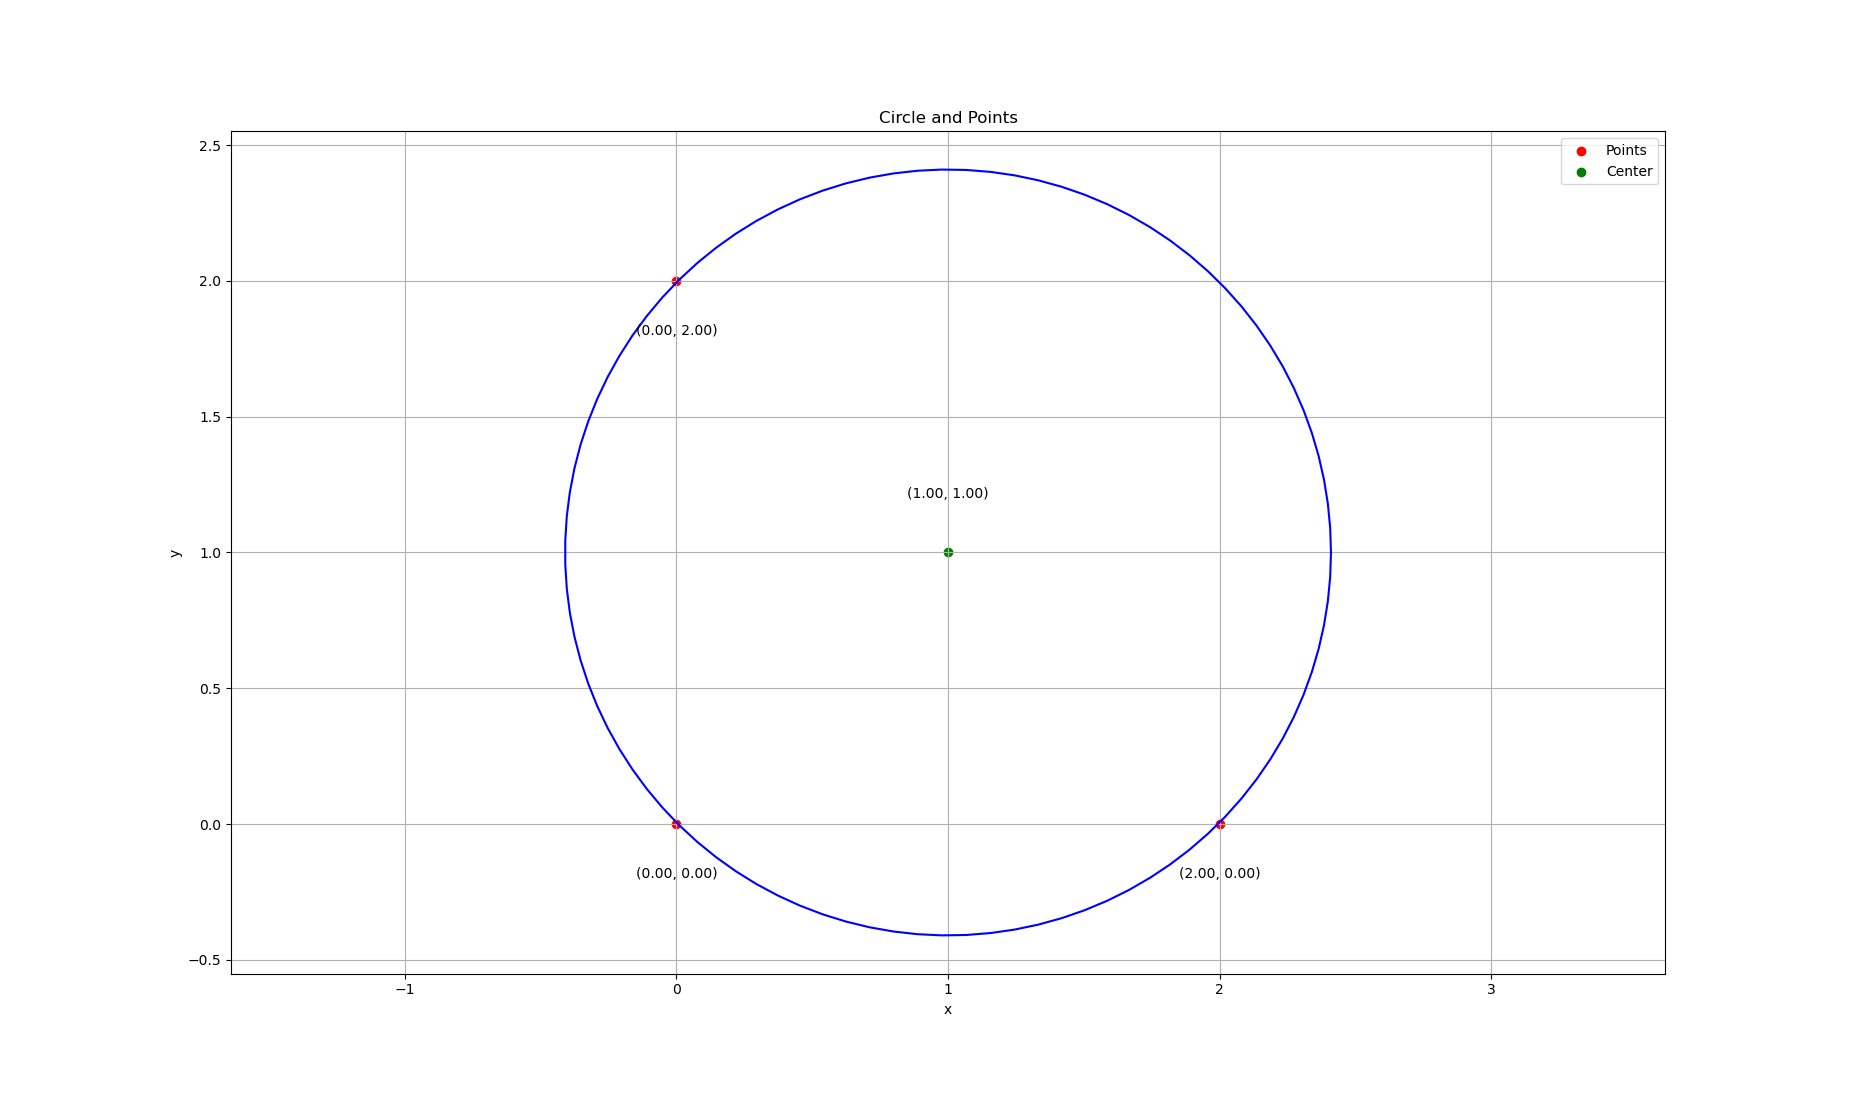
\includegraphics[width=0.7\linewidth]{./figs/Figure_1.png}
\end{figure}
\end{frame}
\end{document}
